\section{Entwurf des abzubildenden Geschäftsprozesses}

Das zu implementierende System soll mittels Microservicearchitektur umgesetzt werden. Die einzelnen Services sollen das Saga-Pattern verwenden, um miteinander zu kommunizieren. Fehler in der Geschäftslogik sollen kompensiert werden. Für jeden auszuführenden Schritt soll es also einen kompensierenden Schritt geben. 

\subsection{Geschäftsprozess}

Als abzubildender Geschäftsprozess soll ein Bestell- und Liefervorgang eines Online-Shops dienen. Der Bestellvorgang soll durch das Platzierung einer Bestellung ausgelöst werden. Die Benutzeroberfläche gehört nicht zum Scope des umzusetzenden Systems. 

Als Ausgangspunkt soll folgender Geschäftsprozess dienen:

\begin{figure}[h!]
	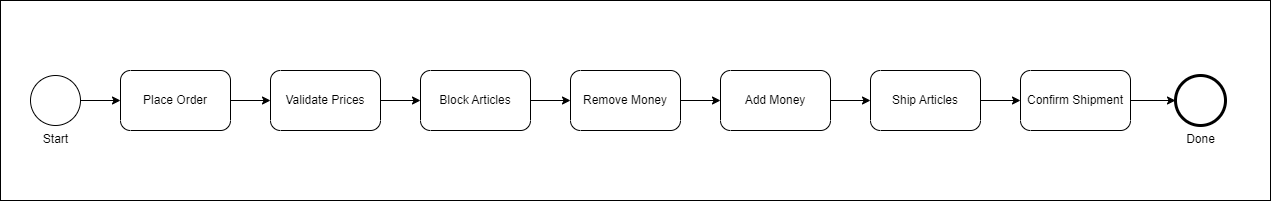
\includegraphics[width=\linewidth]{figures/SimplifiedBusinessProcess.png}
\end{figure}


% TODO Diagramm für den vereinfachten Prozess

Die zum Prozess gehörenden Schritte sind folgende:
\begin{enumerate}
	\item Entgegennehmen der Bestellung: Die Bestellung wird über ein imaginäres Frontend entgegengenommen. Dieses Frontend baut einen Request auf und sendet diesen per Http-Schnittstelle an das Backend. Dort wird der Request entgegengenommen und muss alle für die Abwicklung der Bestellung erforderlichen Daten enthalten. Dazu gehören der bestellende Nutzer, die geforderten Artikel und die Zahlungsinformationen. Beim Entgegennehmen wird die Bestellung initialisiert.
	\item Validierung des Preises: Der Bestellungsrequest enthält eine Liste von den gewünschten Produkten und dem bekannten Preis pro Produkt. Um zu überprüfen, ob der dem Nutzer (dem Frontend) bekannte Preis mit dem aktuellen Preis übereinstimmt, muss dieser validiert werden. % TODO warum ist dieser Schritt notwendig	
	\item Blockieren der Artikel: Die geforderten Artikel sollten für diese Bestellung reserviert werden, bis der Bestellvorgang abgeschlossen ist. In einem Online-Shop wird angezeigt, wieviele Artikel auf Lager vorrätig sind. Beim Blockieren der Artikel wird dieser Betrag verändert. Somit sehen andere Nutzer nach Ausführung dieses Schrittes den aktuellen Wert der vorrätigen Artikel. 
	\item Zahlungsabwicklung: Der berechnete Preis der Bestellung muss vom Konto des Kunden abgebucht und auf das Konto des Händlers gutgeschrieben werden. Die Konten des Kunden und des Online-Shop-Besitzers müssen nicht bei derselben Bank liegen. In diesem Schritt muss also eine verteilte Transaktion stattfinden.
	\item Auslösen der Lieferung: Die blockierten Artikel werden versendet. Dieser Prozess dauert einen längeren Zeitraum an.
	\item Abschluss der Lieferung: Die Saga ist abgeschlossen.
\end{enumerate}

\subsection{Services}
Aus der Beschreibung des Geschäftsprozesses lassen sich folgende Services ableiten:

\begin{center}
	\begin{tabular}[h]{|p{3cm}|p{12cm}|}
		\hline
		Name des Services & Aufgabe \\ \hline
		Frontend & GUI, Anzeige der Produkte, Aufnahme der Bestellung, Platzieren der Bestellung \\ \hline
		OrderService & Entgegennehmen der Bestellung, Koordinierung des Bestellprozesses \\ \hline
		ArticleService & API für die angebotenen Produkte und Preise \\ \hline
		StockService & Informationen über Lagerstand, Auslösen des Lieferprozesses \\ \hline
		BankingServices & Schnittstellen für das Erhöhen und Verringern von Geldbeträten eines Kontos \\ \hline
	\end{tabular}
\end{center}

\subsection{Transaktionen}
Sieht man den gesamten Geschäftsprozess als Transaktion, wären folgende lokale Transaktionen Teil der globalen Transaktion, die durch das Platzieren der Bestellung ausgelöst werden:
\begin{enumerate}
	\item $T_1$: OrderService - Initialisieren der Bestellung
	\item $T_2$: OrderService, ArticleService - Abfragen und Validieren des Preises für jeden geforderten Artikel 
	\item $T_3$: StockService - Blockieren der Artikel
	\item $T_4$: BankingService des Kundenkontos - Verringern des Geldbetrages des Kundenkontos
	\item $T_5$: BankingService des Händlerkontos - Erhöhen des Geldbetrages des Händlerkontos
	\item $T_6$: StockService - Lieferung auslösen
	\item $T_7$: StockService - Lieferung bestätigen
\end{enumerate}

Nach der Funktionsweise des Saga-Patterns muss für jede lokale Transaktion eine Kompensierung angeboten werden:

\begin{center}
	\begin{tabular}[h]{|p{3cm}|p{9.5cm}|}
		\hline
		Transaktion & Kompensierung \\ \hline
		$T_1$ & \\ \hline
		$T_2$ & \\ \hline
		$T_3$ & $C_3$: StockService - Freigeben der Artikel \\ \hline
		$T_4$ & $C_4$: Erhöhen des Geldbetrages des Kundenkontos \\ \hline
		$T_5$ & $C_5$: Verringern des Geldbetrages des Händlerkontos \\ \hline
		$T_6$ & \\ \hline
		$T_7$ & \\ \hline
	\end{tabular}
\end{center}

\section{Fachliche Kontextabgrenzung}

% TODO der Absatz kann vielleicht weg / wo anders hin
Für die Realisierung des Microservicesystems im Rahmen dieser Arbeit wurde die Orchestrierung gewählt. % TODO Begründung warum
Die Rolle des Koordinators übernimmt der OrderService. Der OrderService übernimmt die Annahme des Bestellprozesses und löst somit die Saga aus. 

\subsection{Frontend}
In einem Online-Shop interagiert der Kunde per Frontend mit der Anwendung. Das Frontend soll übernimmt die grafische Schnittstelle zwischen Backend und dem Nutzer. Dazu gehört vor Allem die Darstellung der Artikel in einer Katalogansicht. Die darzustellenden Daten für eine solche Liste müssen zumindest Artikelbezeichnung und Artikelpreis enthalten. Diese Daten sollten aus einer API für Artikeldaten stammen. Darüber hinaus muss das Frontend einen Prozess unterstützen, in dem der Kunde ein Formular ausfüllt, welches die erforderlichen Daten für das Platzieren einer Bestellung enthält. Dazu gehört ein Warenkorbsystem sowie eine Authorisierung und Authentifizierung der Zahlungsidentität des Kunden. Die Bestellung kann also als Objekt mit folgenden Feldern zusammengefasst werden:
\begin{itemize}
	\item Zahlungsinformationen des Kunden: BankId, UserId
	\item Liste der zu bestellenden Artikel, mit Artikel: ArticleId, ArticlePrice, Amount
\end{itemize}

Dieses Objekt kann an das Backend gesendet werden. 

\subsection{ArticleService}
Dieser Service ist ein Service zum reinen Lesen der Produktdaten. Er soll eine Schnittstelle zur Verfügung stellen, die dem Frontend ermöglicht, den Produktkatalog abzufragen und darzustellen. Das Backend muss außerdem die Möglichkeit haben, die im Request enthaltenen Artikelpreise zu validieren. Dazu benötigt der ArticleService eine Produktdatenbank. Da dieser Service ausschließlich die Produktdaten als Ressource behandelt, kann er RESTful implementiert werden.

\subsection{StockService}
Der Service soll den aktuellen Bestand an vorrätigen Artikeln abbilden. Es soll möglich sein, eine Menge an Artikeln für eine konkrete Bestellung zu reservieren. Eine Reservierung von einer Menge von Artikeln wartet auf die Auslösen der Lieferung.

Um dies zu erlauben, muss der aktuelle Lagerstand in einer Tabelle hinterlegt sein. Die Tabelle muss den aktuell verfügbaren Bestand pro Artikel ausdrücken. 

Um eine Reservierung zu ermöglichen, muss es eine weitere Tabelle geben, die eine Menge von blockierten Artikeln für einen bestimmten Bestellprozess enthält. Beim Reservieren verringert sich der Bestand in der Bestandstabelle und erhöht sich in der Reservierungstabelle. Um die Konsistenz zu gewährleisten, müssen beide Operationen in einer lokalen Transaktion ausgeführt werden. 

Um das Auslösen und Abschließen einer Lieferung zu ermöglichen, muss es eine Tabelle geben, die den Inhalt einer Lieferung und einen Status enthält.
Wenn eine Lieferung ausgelöst wird, werden die für diesen Vorgang reservierten Artikel aus der Reservierungstabelle entfernt und in der Lieferungstabelle eingefügt. Diese Transaktion soll den physischen Prozess abbilden, die bestellten und für diese Bestellung blockierten Artikel aus dem Lager in das Transportfahrzeug und schließlich zum Kunden zu transferieren.

Die Übergabe der Ware an den Kunden stellt den finalen Schritt des Prozesses dar. Ist dies geschehen, gibt der Lieferant dem StockService die Bestätigung für die gelieferte Bestellung.

Die Blockierung eines Artikels muss kompensiert werden können, da sonst der reservierte Artikel nach Abbruch einer Bestellung nicht wieder freigegeben würde. Deshalt muss diese Kompensierung die Einträge aus der Blockierungstabelle entfernen und die Anzahl auf den Lagerbestand addiert werden. Dies soll ebenfalls in einer lokalen Transaktion ablaufen, um Konsistenz zu wahren.

Die Auslösung der Lieferung ist nur bedingt kompensierbar. Nachdem das Transportfahrzeug mit der Ware losgefahren ist und die Ware noch nicht übergeben hat, kann die Lieferung noch abgebrochen und somit kompensiert werden. Die Kompensierung muss also den Lieferant benachrichtigen und die Ankunft der Waren bestätigen. Nach der Saga-Definition soll die zu kompensierende Transaktion zurückgerollt werden. Deshalb werden die Waren aus der Lieferungstabelle zurück in die Reservierungstabelle geschrieben. 

Der Abschluss einer Lieferung bildet die physische Warenübergabe an den Kunden ab. Eine Kompensierung ist hier nicht möglich. Da diese lokale Transaktion die letzte Transaktion ist und einen erfolgreichen Abschluss der Saga zur Folge hat, muss hier keine Kompensierung angeboten werden.

\subsection{BankingServices}
Im Geschäftsprozess wurde definiert, dass die Transaktion den Geldbetrag des Kundenkontos und des Händlerkontos in zwei separaten lokalen Transaktionen abwickeln können soll. Somit muss der BankingService jeweils eine Transaktion zum Erhöhen und zum Verringern des Geldbetrages anbieten. Der BankingService soll am Ende in zwei Instanzen laufen, die zwei verschiedene Banken darstellen sollen. Kunden- und Käuferkonto können, müssen aber nicht bei derselben Bank liegen. 

Um dies zu ermöglichen benötigt der BankingService eine Tabelle, die seine Nutzer enthält. Zusätzlich benötigt der Service eine Tabelle, die den aktuellen Geldbetrag jedes Nutzers enthält. Außerdem sollten die einzelnen Transaktionen jedes Nutzers in einer separaten Tabelle gesichert werden. Für die reine Implementierung dieser Anwendung wäre dies nicht notwendig. Für den Nutzer eines BankingServices ist neben dem Kontostand auch die Liste an getätigten Transaktionen interessant, um die Ausgaben und Einnahmen zuordnen zu können. Im Rahmen dieser Implementierung wird die Tabelle zusätzlich für Analysezwecke verwentet werden.
 
Bei einer Anfrage, den Geldbetrag eines konkreten Nutzers zu erhöhen, wird in einer lokalen Transaktion der Betrag des Kontos in der UserCredit-Tabelle erhöht und die Differenz in der Transaktion-Tabelle eingetragen. 

Der Service muss Anfragen zum Geldabbuchung ablehnen, wenn die Verringerung den Kontostand in den negativen Bereich fallen lassen würde. In diesem Fall wird die Transaktion abgebrochen.

Beide angebotenen Operationen benötigen eine zugehörige Kompensation, da sie den Datenbestand verändern. Die Verwendung des jeweils anderen Endpunktes ist semantisch bereits korrekt. Der Klarheit halber sollen zwei weitere Entpunkte eingeführt werden, die nur für die Kompensation verwendet werden sollen.

\subsection{OrderService}
Der OrderService übernimmt die Rolle des Koordinators im Orchestrator-Saga-Patterns. Die Bestellung wird entgegengenommen und vom OrderService initialisiert. Zur Initialisierung gehört die Generierung einer Vorgangsnummer sowie das Abspeichern der Bestellung in einer separaten Tabelle. Anhand dieser Tabelle wird persistiert, an welcher Stelle der Ausführung die Saga sich befindet, und in welchem Status die Bestellung ist. Die etwaigen ausgeführten Kompensationsschritte sind in ihrer eigenen Tabelle und werden der Vorgansnummer zugeordnet. Die gewünschten Artikel einer Bestellung sind in eine separate Tabelle ausgelagert und verweisen auf die Saga-Tabelle. 

Als Koordinator hat dieser Service die Verantwortung, die an der Saga beteiligten Services korrekt aufzurufen. Die Reihenfolge und die getroffenen Entscheidungen repräsentieren die Geschäftslogik. 

Nach jedem Schritt persistiert der OrderService den Erfolg oder Misserfolg. Die Tabelle, in der die Schritte gespeichert werden, stellt das Saga Execution Log dar. Außerdem ruft der Service nach Feststellung eines Misserfolgs die Backward-Recovery auf. 

Neben der Schnittstelle zum Platzieren der Bestellung soll dem Nutzer ermöglicht werden, die Bestellung zu stornieren. Dieser zusätzliche Endpunkt nimmt die Vorgangsnummer der zuvor ausgelösten Bestellung entgegen. Falls die Ware noch nicht beim Kunden eingetroffen ist, kann hier die Bestellung abgebrochen werden. Eine solche Stornierung löst ebenfalls Backward-Recovery aus und soll den Initialzustand wiederherstellen. Diese Aktion stellt keine lokale Transaktion der globalen Transaktion dar; es ist eine Aktion, die von außen in den Bestellprozess eingreift. Damit ist die Stornierung kein T und hat somit kein zugehöriges C.

% Tabellen, Transaktionen, Endpunkte
\section{Technische Kontextabgrenzung}
% TODO Quelle Database per Service vs Shared Database
Bei der Modellierung der Datenbankschicht wurde das Database-per-Service Muster verwendet. Dieses Muster erlaubt eine sehr lose Bindung der Services und lässt die Datenbasis in der Verantwortung eines Services. Es ist möglich, ein Microservice-System zu implementieren, welches das Muster einer gemeinsamen Datenbank verwendet. Dies würde die Implementierung atomaren und konsistenten Transaktionen vereinfachen. Die Voraussetzungen für eine solche Implementierungen sind jedoch nicht immer gegeben, da an der LLT teilhabende Services unter Umständen nicht in der Verantwortung des Entwicklerteams liegen könnten, welches die LLT zu implementieren hat. Aus diesem Grund wird im Rahmen der für diese Implementierung vorzunehmende Implementierung jeder Service als getrennte Komponente aufgefasst, die als alleinige Instanz auf ihre eigenen Daten zugreift und zugreifen kann.

% TODO vereinfachte Darstellung der Schnittstellen im folgenden, ausführliche Beschreibung in Swaggerfile im Anhang

\subsection{ArticleService}
\subsubsection{Datenbankschicht}

Der ArticleService soll lediglich Daten aus der Datenbanksicht zurückliefern. Deshalb wird für diesen Service lediglich eine Tabelle benötigt. Die Tabelle $article$ enthält für jeden anzubietenden Artikel den zugehörigen Namen und Preis.

\begin{figure}[h!]
	\centering
	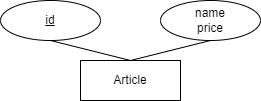
\includegraphics[scale=0.5]{figures/DatabaseER/ArticleServiceTables.png}
	\caption{ER-Diagramm ArticleService}
\end{figure}
\FloatBarrier

\subsubsection{Schnittstellen} % TODO RESTful, Ressource
Die Produktdaten sollen von dem Frontend abgefragt und dargestellt werden. Dabei werden alle vorhandenen Produktdaten selektiert und zurückgegeben. 

Zusätzlich soll der Koordinator eine gezielte Abfrage durchführen können, welche den Preis eines Artikels für eine gegebene ProduktId liefert. Beide Schnittstellen sind RESTful, da jeder Artikel als Ressource angesehen wird. 

\begin{center}
	\begin{tabular}[h]{|p{3.5cm}|p{3cm}|p{2cm}|}
	\hline
	Endpunkt & Http-Methode & Argumente \\ \hline
	/api/articles & GET & \\ \hline
	/api/articles/\{id\} & GET & ArticleId \\ \hline
\end{tabular}
\end{center}
\FloatBarrier

\subsubsection{Mögliche Antwortmöglichkeiten}
Die Schnittstelle  $/api/arcicles$ liefert die Produktdaten im Response-Body und antwortet mit einem Statuscode von $200, OK$. Es gibt hier keine möglichen Fehlerquellen, weshalb keine weiteren Antwortmöglichkeiten infrage.

Die Schnittstelle $/api/articles/\{id\}$ sucht in der Datenbank gezielt nach dem Artikel mit der geforderten Id. Im Erfolgsfall antwortet die Schnittstelle ebenfalls mit $200, OK$. Wird der Artikel nicht gefunden, erfolgt die Antwort mit Statuscode $404, Not Found$.

\subsection{StockService}
\subsubsection{Datenbankschicht}

Der StockService verwaltet vier Tabellen. Die zentrale Tabelle ist $articlestock$ und stellt für jeden bekannten Artikel den auf Lager befindlichen Vorrat dar. Eine Reservierung für eine gegebene Vorgangsnummer wird in der Tabelle $blockedarticles$ durch alle Tupel, bei denen diese Nummer auftritt. Die Lieferungen werden in der Tabelle $shipments$ dargestellt. Auch hier gehört eine Vorgangsnummer zu den Spalten. Zusätzlich gibt es das Attribut $hasarrived$, was Auskunft über den Status der Lieferung gibt. Die zu einer Lieferung gehörenden Artikel und deren Menge sind in der Tabelle $shippedarticles$ enthalten.

\begin{figure}[h!]
	\centering
	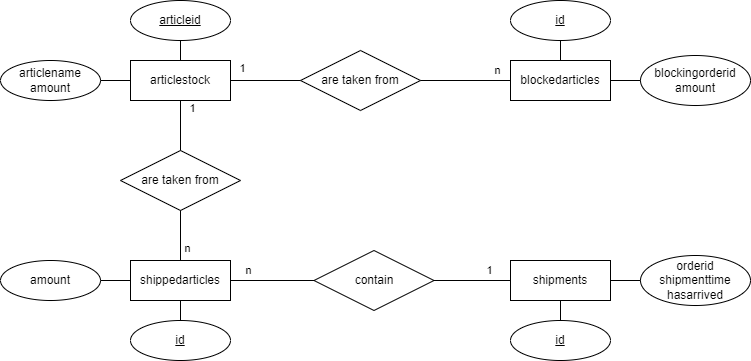
\includegraphics[scale=0.5]{figures/DatabaseER/StockServiceTables.png}
	\caption{ER-Diagramm StockService}
\end{figure}
\FloatBarrier

\subsubsection{Schnittstellen}

Der Endpunkt $/api/blocked-articles$ überträgt frei verfügbare Artikel aus der Tabelle $articlestock$ in die Tabelle $blockedarticles$. Als Argumente werden die zu blockierenden Artikel-Ids und Artikel-Mengen sowie die Vorgangsnummer benötigt. Teil der lokalen Transaktion sind folgende Schritte:
\begin{enumerate}
	\item Reduzieren jedes Artikelvorrats in der Tabelle $articlestock$
	\item Einfügen eines Elements in der Tabelle $blockedarticles$ für jede zu blockierende Artikel-Id
\end{enumerate}

Der Endpunkt $/api/blocked-articles-compensation$ stellt die Kompensierung für die Schnittstelle $/api/blocked-articles$ dar. Als Argument wird hier lediglich die Vorgangsnummer benötigt. Notwendige Schritte der auszuführenden lokalen Transaktion sind:
\begin{enumerate}
	\item Selektieren aller Elemente aus $blocked-articles$ mit der angefragten Vorgangsnummer
	\item Löschen dieser Elemente
	\item Erhöhen der Vorratsmengen in $articlestock$ für jede Artikelblockierunge
\end{enumerate}

Der Endpunkt $/api/start-shipment$ erwartet die Vorgangsnummer als Argument. Die reservierten Artikel werden in eine Lieferung umgewandelt und versendet. Die Schritte der ablaufenden lokalen Transaktion sind:
\begin{enumerate}
	\item Initialisieren eines Elements in $shipments$ mit dem Status $hasarrived=0$
	\item Selektieren und Löschen aller Elemente in $blockedarticles$, die die OrderId enthalten
	\item Einfügen der Selektierungen in der Tabelle $shippedarticles$
\end{enumerate}

Der Endpunkt $/api/finish-shipment$ wird ausschließlich vom Lieferanten verwendet und dient zur Bestätigung der Lieferung. Es wird lediglich der Status der entsprechenden ShipmentId in der Tabelle $shipments$ auf 1 gesetzt.

Der Endpunkt $/api/shipments$ liefert lediglich den Status der angeforderten ShipmentId. Der Koordinator hat mit dem Aufruf von $/api/start-shipments$ die Lieferung ausgelöst. Der Koordinator hat mit der Schnittstelle $/api/shipments$ die Möglichkeit, den Status der Lieferung solange abzufragen, bis der Lieferant per Aufruf von $/api/finish-shipment$ den Lieferabschluss bestätigt. Die Kombination von $/api/start-shipment$, $/api/finish-shipment$ und $/api/shipments$ können als Polling-Implementierung eines asynchronen Request-Response Musters aufgefasst werden. 

Der letzte Endpunkt des StockServices ist $/api/cancel-shipment$ und bietet dem Koordinator die Möglichkeit, auf eine Stornierung zu reagieren. Bis die Lieferung abgegeben und bestätigt wurde, kann diese Schnittstelle verwendet werden, um die Lieferung abzubrechen. Als Argument wird die ShipmentId benötigt.

\begin{center}
	\begin{tabular}[h]{|p{4.5cm}|p{1.5cm}|p{5.5cm}|}
		\hline
		Endpunkt & Http-Methode & Argumente \\ \hline
		/api/blocked-articles & POST & ArticleId, Amount, OrderId\\ \hline
		/api/blocked-articles-compensation & POST & OrderId \\ \hline
		/api/start-shipment & POST & OrderId \\ \hline
		/api/finish-shipment & POST & ShipmentId \\ \hline
		/api/shipments & GET & ShipmentId \\ \hline
		/api/cancel-shipment & POST & ShipmentId \\ \hline
	\end{tabular}
\end{center}
\FloatBarrier

\subsubsection{Mögliche Antwortmöglichkeiten}
Für $/api/blocked-articles$ antwortet im Erfolgsfall mit einem $200, OK$. 

\subsection{BankingService}
\subsubsection{Datenbankschicht} % TODO Tabellenbezeichnungen anpassen
Zur Verwaltung des BankingServices gehören drei Tabellen. Die Tabelle $bankuser$ enthält alle Nutzer, die Tabelle $bankusercredit$ ordnet jedem Nutzer einen Kontostand zu und die Tabelle $bankusertransaction$ stellt Veränderung des Kontostands der Tabelle $bankcredit$ in der Tabelle $bankusertransaction$ als Historie dar.

\begin{figure}[h!]
	\centering
	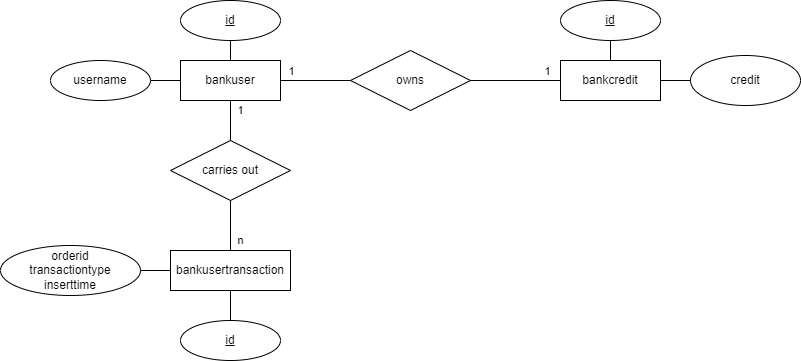
\includegraphics[scale=0.5]{figures/DatabaseER/BankingServiceTables.png}
	\caption{ER-Diagramm BankingService}
\end{figure}
\FloatBarrier

\subsubsection{Schnittstellen}
Der BankingService bietet jeweils eine Schnittstelle zum Erhöhen und zum Verringern des Kontostandes an. Dabei wird lediglich in der Tabelle $bankcredit$ das Credit-Attribut erhöht oder verringert. Die Spalte ist im Datenbankmanagementsystem mit einer Einschränkung versehen, die verhindert, dass der Wert der Spalte unter 0 fällt. 

Die Veränderung des Kontostandes ist der erste Schritt der lokalen Transaktion. Der zweite Schritt ist das Einfügen eines neuen Elementes in der Tabelle $bankusertransaction$. In dieser Tabelle wird der Transaktionstyp festgehalten, der den Typ

\begin{center}
	\begin{tabular}[h]{|l|l|l|}
		\hline
		Endpunkt & Http-Methode & Argumente \\ \hline
		/api/add-money & POST & UserId, Amount, OrderId \\ \hline
		/api/add-money-compensation & POST & UserId, Amount, OrderId \\ \hline
		/api/remove-money & POST & UserId, Amount, OrderId \\ \hline
		/api/remove-money-compensation & POST & UserId, Amount, OrderId \\ \hline 
	\end{tabular}
\end{center}
\FloatBarrier

\section{Darstellung als DEA}
Der entworfene Prozess soll nun als DEA dargestellt werden. Dafür sind alle möglichen Ergebnisse zu erfassen, die jede lokale Transaktion aus Sicht des Koordinators liefern kann. 
Für die Ts ergeben sich folgende Ergebnisse:

\begin{center}
	\begin{tabular}[h]{|p{3cm}|p{1.5cm}|p{11cm}|}
		\hline
		Transaktion	& Ergebnis & Bedeutung \\ \hline
		Initialize Saga 	& Success 	& Bestellung ist initialisiert \\ \hline
		Get Article Data	& 200 		& Artikeldaten wurden vom ArticleService empfangen \\
							& 404 		& Artikel wurde nicht gefunden \\ \hline
		Validate Price 		& Success 	& Preis aus Bestellung und aus dem System stimmen überein \\
							& Failure 	& Preise aus Bestellung und aus dem System stimmen nicht überein \\ \hline
		Block Articles		& 200		& Produkte wurden reserviert \\
							& 409 		& Lagervorrat ist erschöpft \\
							& 429 		& Mehrere Transaktionen behindern sich und lokale Transaktion schlägt fehl \\ \hline
		Remove Money 		& 200		& Geldbetrag auf dem Konto wurde verringert \\
							& 404		& Nutzer wurde nicht gefunden \\
							& 409		& Lokale Transaktion ist fehlgeschlagen (Konto ist nicht gedeckt) \\
							& 429		& Mehrere Transaktionen behindern sich und lokale Transaktion schlägt fehl \\ \hline
		Add Money 			& 200		& Geldbetrag auf dem Konto wurde erhöht \\
							& 404		& Nutzer wurde nicht gefunden \\
							& 409		& Lokale Transaktion ist fehlgeschlagen \\
							& 429		& Mehrere Transaktionen behindern sich und lokale Transaktion schlägt fehl \\ \hline
		Start Shipment 		& 200		& Lieferung wurde ausgelöst \\
							& 404		& Zur geforderten Bestellnummer wurde keine Reservierung gefunden \\
							& 409		& Lokale Transaktion ist fehlgeschlagen \\
							& 429 		& Mehrere Transaktionen behindern sich und lokale Transaktion schlägt fehl \\ \hline
		Check Cancellation 	& Success	& Es wurde keine Stornierung festgestellt \\
							& Failure	& Es wurde eine Stornierung festgestellt \\ \hline
		Get Shipment Status	& 200 		& Status wurde vom StockService empfangen \\
							& 404		& Lieferung existiert nicht \\ \hline
		Check Shipment Status& Success	& Lieferstatus signalisiert abgeschlossene Lieferung \\
							& Failure 	& Lieferstatus signalisiert noch nicht abgeschlossene Lieferung \\ \hline
	\end{tabular}
\end{center}
\FloatBarrier

Für die Cs ergeben sich folgende Ergebnisse:
\begin{center}
	\begin{tabular}[h]{|p{5.5cm}|p{1.5cm}|p{8.5cm}|}
		\hline
		Transaktion 						& Ergebnis 	& Bedeutung \\ \hline
		Initialize Saga Compensation	 	& Success 	& \\ \hline
		Get Article Data Compensation	 	& Success 	& \\ \hline	
		Validate Price Compensation	 		& Success 	& \\ \hline
		Block Articles Compensation	 		& 200	 	& Reservierung wurde aufgehoben \\
											& 409		& Lokale Transaktion ist fehlgeschlagen \\
											& 429 		& Mehrere Transaktionen behindern sich und lokale Transaktion schlägt fehl \\ \hline
		Remove Money Compensation		 		& 200		& Geldbetrag auf dem Konto wurde erhöht \\
											& 404		& Nutzer wurde nicht gefunden \\
											& 409		& Lokale Transaktion ist fehlgeschlagen \\
											& 429		& Mehrere Transaktionen behindern sich und lokale Transaktion schlägt fehl \\ \hline
		Add Money Compensation		 		& 200		& Geldbetrag auf dem Konto wurde erhöht \\
											& 404		& Nutzer wurde nicht gefunden \\
											& 409		& Lokale Transaktion ist fehlgeschlagen \\
											& 429		& Mehrere Transaktionen behindern sich und lokale Transaktion schlägt fehl \\ \hline
		Start Shipment Compensation	 		& 200	 	& Lieferung wurde abgebrochen \\
			 								& 404		& Lieferung existiert nicht \\
											& 409		& Lokale Transaktion ist fehlgeschlagen \\
											& 410		& Lieferung wurde nicht abgebrochen, da sie bereits abgeschlossen ist \\
											& 429		& Mehrere Transaktionen behindern sich und lokale Transaktion schlägt fehl \\ \hline
	\end{tabular}
\end{center}
\FloatBarrier

\begin{figure}[h!]
	\centering
	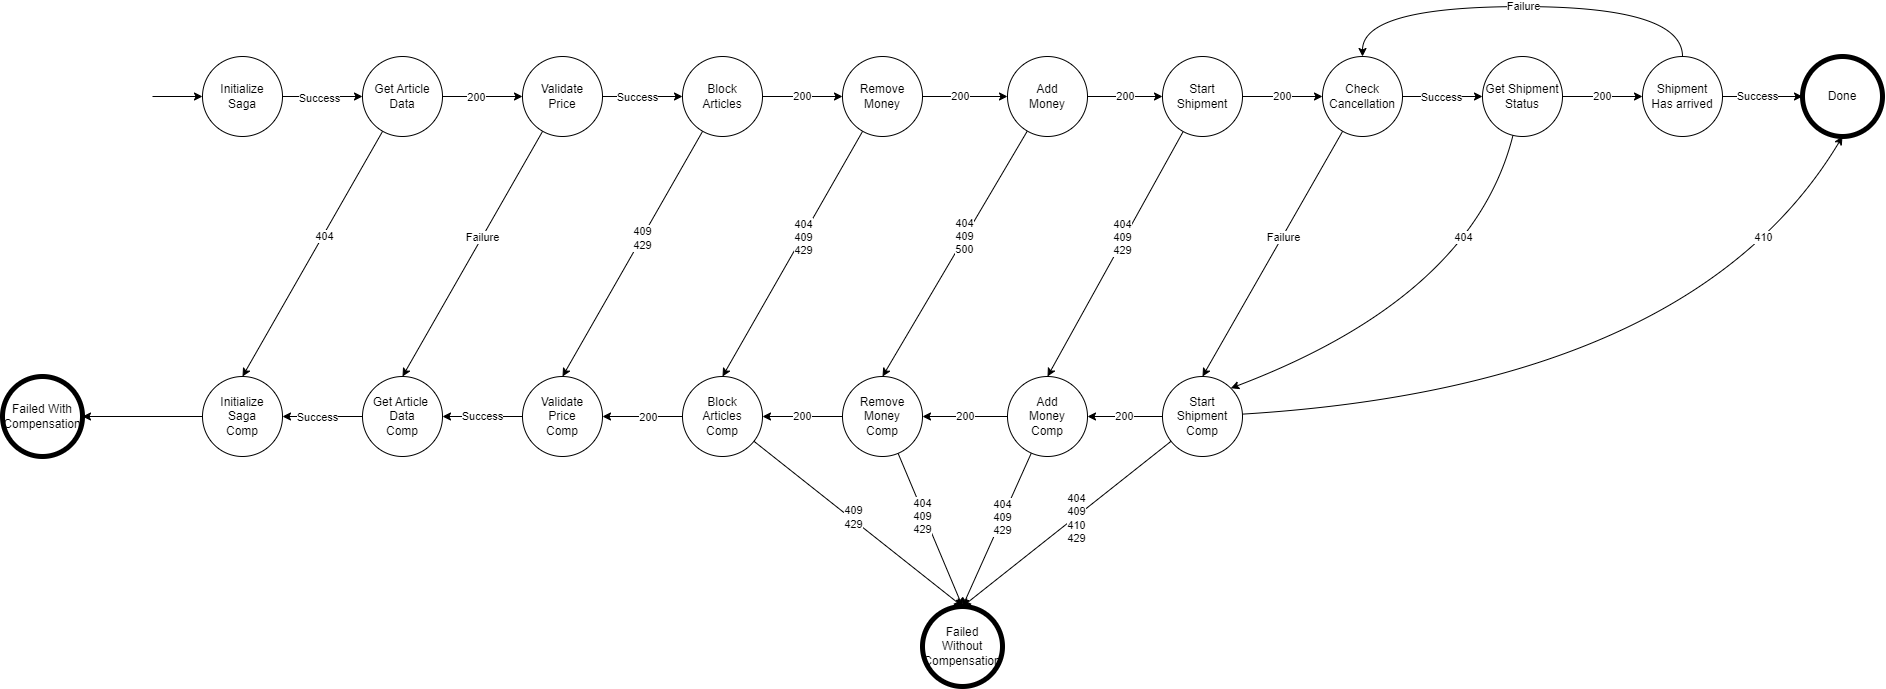
\includegraphics[width=\linewidth]{figures/DatabaseER/DEA_No_NetworkErrors_No_Retries.png}
	\caption{Saga als DEA}
\end{figure}
\FloatBarrier


\subsubsection{Durchlauf einer erfolgreichen Saga}
% TODO Ablaufdiagramm mit nummerierten Pfeilen

\subsubsection{Durchlauf einer gescheiterten, kompensierten Saga}
% TODO Ablaufdiagramm mit nummerierten Pfeilen

\subsubsection{Durchlauf einer gescheiterten, nichtkompensierten Saga}
% TODO Ablaufdiagramm mit nummerierten Pfeilen